\documentclass{article}

\usepackage{ctex}
\usepackage{anyfontsize}
\usepackage{amsfonts}
\usepackage{amsmath}
\usepackage{amsthm}
\usepackage{amssymb}
\usepackage{graphicx}
\usepackage{float}
\usepackage{hyperref}
\usepackage{mathabx}
\usepackage{datetime}
\usepackage{tabularray}
\usepackage{geometry}
\usepackage{centernot}
\usepackage[dvipsnames]{xcolor}

\title{高等数学}
\author{}
\date{\today}

\geometry{a4paper,scale=0.8}

\begin{document}

\hypersetup{
    hidelinks,
    %colorlinks = true,
    allcolors = black,
    %pdfstartview = Fit,
    breaklinks = true
}

\newtheorem{definition}{Definition}[subsection]
\newtheorem{theorem}{Theorem}[subsection]
\newtheorem{corollary}{Corollary}[theorem]
\renewcommand{\proofname}{\indent\bf Proof}
\renewcommand{\Re}{\operatorname{Re}}
\renewcommand{\Im}{\operatorname{Im}}
\numberwithin{equation}{section}

\def\e{\mathrm e}
\def\i{\mathrm i}
\def\d{\mathrm d}
\def\C{\mathrm C}
\def\sr{\mathbb R}
\def\sn{\mathbb N}
\def\snp{\mathbb N^+}
\def\sc{\mathbb C}
\def\sz{\mathbb Z}
\def\sech{\mathrm{sech}}
\def\csch{\mathrm{csch}}

\newcommand{\abs}[1]{\left|#1\right|}
\newcommand{\p}[1]{\left(#1\right)}
\newcommand{\jacobi}[2]{\frac{\partial\p{#1}}{\partial\p{#2}}}

\begin{titlepage}
    \maketitle
\end{titlepage}

\tableofcontents
\newpage

\part{极限}

\section{基础}

\subsection{常用极限}

\[\begin{aligned}
         & \lim_{x\to0^+}{\p{1+\frac1x}^x}                     &  & =1                              \\
         & \lim_{x\to\infty}{\p{1+\frac1x}^x}                  &  & =\e                             \\
         & \lim_{n\to\infty}{\frac1n\sum_{i=1}^nf\p{\frac in}} &  & =\int_0^1f\p{x}\d x\p{n\in\snp} \\
         & \lim_{n\to\infty}{\sqrt[n]{\sum a_i^n}}             &  & =\max{\left\{a_i\right\}}
    \end{aligned}\]

\subsection{常用等价无穷小}

$x$为函数,$\lim\limits_{x\to0}$时,可对乘除因子替换

\[x\sim\sin x\sim\tan x\sim\arcsin x\sim\arctan x\]

\[x\sim\p{\e^x-1}\sim\ln\p{x+1}\sim\ln\p{x+\sqrt{1+x^2}}\]

\[x^3\sim6\p{x-\sin x}\sim6\p{\arcsin x-x}\sim3\p{\tan x-x}\]

\[x^3\sim3\p{x-\arctan x}\sim2\p{\tan x -\sin x}\]

\[\begin{aligned}
         & 1-\cos x            &  & \sim\frac{x^2}2                    \\
         & \log_a{\p{1+x}}     &  & \sim\frac x{\ln a}                 \\
         & \p{1+x}^a           &  & \sim ax+1                          \\
         & a^x-1               &  & \sim x\ln a\p{0<a\neq1}            \\
         & \p{1+ax}^\frac1{bx} &  & \sim\e^\frac ab(1-\frac{a^2}{2b}x) \\
    \end{aligned}\]

\subsection{泰勒展开}

详见\ref{Taylor}

\section{间断点}

\subsection{第一类间断点}

\[\exists\lim_{x\to x_0^-}\text{且}\exists\lim_{x\to x_0^+}\]

\subsubsection{可去间断点}

\[\lim_{x\to x_0^-}f\p{x}=\lim_{x\to x_0^+}f\p{x}=A\p{\iff\lim_{x\to x_0}f\p{x}=A}\]

\subsubsection{跳跃间断点}

\[\lim_{x\to x_0^-}f\p{x}\neq\lim_{x\to x_0^+}f\p{x}\]

\subsection{第二类间断点}

\[\lim_{x\to x_0^-},\lim_{x\to x_0^+}\text{至少满足有一个}\nexists\]

\subsubsection{振荡间断点}

左、右极限至少一个为振荡不存在

\subsubsection{无穷间断点}

左、右极限至少一个为$\infty$

\section{洛必达法则}

\subsection{使用条件}

\paragraph{定义存在}

\[x\in\mathring{U}\p{x_0}\text{(}x_0\text{可取}\infty\text{)},
    \exists f^\prime\p{x_0},
    \exists g^\prime\p{x_0}\]

\paragraph{极限存在或为无穷}

\[g^\prime\p{x_0}\neq0,\exists\lim_{x\to x_0}\frac{f^\prime\p{x}}{g^\prime\p{x}}\text{或}=\infty\]

\paragraph{符合$\dfrac00$或$\dfrac{\text{任意}}{\infty}$}

\subsection{结论}

\[\begin{aligned}
        \lim_{x\to x_0}\frac{f^\prime\p{x}}{g^\prime\p{x}}=A       & \implies\lim_{x\to x_0}\frac{f\p{x}}{g\p{x}}=A                 \\
        \lim_{x\to x_0}\frac{f^\prime\p{x}}{g^\prime\p{x}}=\infty  & \implies\lim_{x\to x_0}\frac{f\p{x}}{g\p{x}}=\infty            \\
        \nexists\lim_{x\to x_0}\frac{f^\prime\p{x}}{g^\prime\p{x}} & \centernot\implies\nexists\lim_{x\to x_0}\frac{f\p{x}}{g\p{x}}
    \end{aligned}\]

\section{极限审敛}

\subsection{单调有界准则}

单调有界必有极限

\subsection{一类二重极限}

\[\lim_{\substack{x\to0^+ \\ y\to0^+}}\frac{x^py^q}{x^m+y^n}\]

$m$、$n$全为偶数且$\dfrac pm+\dfrac qn>1$时$\lim\limits_{\substack{x\to0^+ \\ y\to0^+}}\dfrac{x^py^q}{x^m+y^n}=0$,否则不存在

$\dfrac pm+\dfrac qn\leqslant1$时,路径$y=kx^{\frac{m-p}q}$可说明极限不存在

\part{导数}

\section{基础}

\subsection{定义}

\[f^\prime\p{x_0}=\lim_{x\to x_0}\frac{f\p{x}-f\p{x_0}}{x-x_0}\]

\subsection{求导法则}

\[\begin{aligned}
        \p{f\p{x}+g\p{x}}^\prime                      & =f^\prime\p{x}+g^\prime\p{x}                                         \\
        \p{f\p{x}g\p{x}}^\prime                       & =f\p{x}g^\prime\p{x}+f^\prime\p{x}g\p{x}                             \\
        \p{f\p{g\p{x}}}^\prime                        & =f^\prime\p{g\p{x}}g^\prime\p{x}                                     \\
        \p{\int_{v\p{x}}^{u\p{x}}f\p{t}\d t}^\prime   & =f\left[u\p{x}\right]u^\prime\p{x}-f\left[v\p{x}\right]v^\prime\p{x} \\
        \p{\int_{v\p{x}}^{u\p{x}}f\p{x,t}\d t}^\prime & =\int_{v\p{x}}^{u\p{x}}f_x^\prime\p{x,t}\d t
        +f\left[x,u\p{x}\right]u^\prime\p{x}-f\left[x,v\p{x}\right]v^\prime\p{x}
    \end{aligned}\]

\subsection{常用高阶导数}

\[\begin{aligned}
         & \sin^{\p{n}}\omega x &  & =\omega^n\sin\p{\omega x+\frac{n\pi}2}   &  & \p{n\in\sn}  \\
         & \cos^{\p{n}}\omega x &  & =\omega^n\cos{\p{\omega x+\frac{n\pi}2}} &  & \p{n\in\sn}  \\
         & \ln^{\p{n}}\p{1+x}   &  & =\p{-1}^{n-1}\frac{\p{n-1}!}{\p{1+x}^n}  &  & \p{n\in\snp} \\
         & \ln^{\p{n}}\p{1-x}   &  & =-\frac{\p{n-1}!}{\p{1-x}^n}             &  & \p{n\in\snp} \\
    \end{aligned}\]

\subsection{极值和凹凸}

\subsubsection{一般情况}

\[\begin{aligned}
        f^\prime\p{x_0}>0         & \implies x_0\text{处是单调递增的}\nearrow \\
        f^\prime\p{x_0}<0         & \implies x_0\text{处是单调递减的}\searrow \\
        f^{\prime\prime}\p{x_0}>0 & \implies x_0\text{处是凹的}            \\
        f^{\prime\prime}\p{x_0}<0 & \implies x_0\text{处是凸的}
    \end{aligned}\]

极值点处可以不连续

拐点处必须连续

\subsubsection{必要条件}

\[\begin{aligned}
         & x_0\text{是极值点},f^\prime\p{x}\exists        & \implies & f^\prime\p{x_0}=0         \\
         & x_0\text{是拐点},f^{\prime\prime}\p{x}\exists & \implies & f^{\prime\prime}\p{x_0}=0
    \end{aligned}\]

\subsubsection{充分条件1}

$f^\prime\p{x_0}$在$x_0$两侧异(同)号$\implies x_0$是(不是)极值点

$f^{\prime\prime}\p{x_0}$在$x_0$两侧异(同)号$\implies x_0$是(不是)拐点

\subsubsection{充分条件2}

\[f^\prime\p{x_0}=f^{\prime\prime}\p{x_0}=\cdots=f^{\p{n-1}}\p{x_0}=0,f^{\p{n}}\p{x_0}\neq0\p{n\geqslant2}\]

\[\left\{\begin{aligned}
        n\text{为奇数} & \implies x_0\text{是拐点}  \\
        n\text{为偶数} & \implies x_0\text{是极值点}
    \end{aligned}\right.\]

\subsection{渐近线}

\subsubsection{铅直渐近线}

\[x=x_0\]

\[\lim_{x\to x_0^\pm}f\p{x}=\infty\]

\subsubsection{水平渐近线}

\[y=A\]

\[\lim_{x\to\pm\infty}f\p{x}=A\]

\subsubsection{斜渐近线}

\[y=kx+b\]

\[\lim_{x\to\pm\infty}f\p{x}=kx+b\]

\[\left\{\begin{aligned}
         & \lim_{x\to\pm\infty}\frac{f\p{x}}x=k \\
         & \lim_{x\to\pm\infty}f\p{x}-kx=b
    \end{aligned}\right.\]

\subsection{莱布尼茨公式}

\[\p{uv}^{\p{n}}=\sum_{k=0}^n\binom nku^{\p{n-k}}v^{\p{k}}\]

\subsection{中值定理}

\[\begin{tblr}{c|c|c}
        \hline
        \text{定理}       & \text{公式}                                                                                         & \text{约束}              \\
        \hline
        \text{积分中值定理}   & f\p{\xi}=\dfrac{\int_a^bf\p{x}\d x}{\left.x\right|_a^b}                                           & \xi\in\left[a,b\right] \\
        \text{罗尔中值定理}   & a=b\Rightarrow f^\prime\p{\xi}=0                                                                  & \xi\in\p{a,b}          \\
        \text{拉格朗日中值定理} & f^\prime\p{\xi}=\dfrac{\left.f\p{x}\right|_a^b}{\left.x\right|_a^b}                               & \xi\in\p{a,b}          \\
        \text{柯西中值定理}   & \dfrac{f^\prime\p{\xi}}{g^\prime\p{\xi}}=\dfrac{\left.f\p{x}\right|_a^b}{\left.g\p{x}\right|_a^b} & \xi\in\p{a,b}          \\
        \hline
    \end{tblr}\]

\subsection{泰勒中值定理}

$R_n\p{x}$为余项

\[\begin{aligned}
         & P_n\p{x}   &  & =\sum_{i=0}^n\p{x-x_0}^i\frac{f^{\p{i}}\p{x_0}}{i!}+R_n\p{x}                                                   \\
         & P_n\p{x,y} &  & =\sum_{i=0}^n\left[\p{x-x_0}\partial_x+\p{y-y_0}\partial_y\right]^i\frac{f\p{x_0,y_0}}{i!}+R_n\p{x,y}\label{2}
    \end{aligned}\]

\subsubsection{佩亚诺型余项}

\[\begin{aligned}
        R_n\p{x}   & =
        o\left[\p{x-x_0}^n\right] \\
        R_n\p{x,y} & =
        o\left[\sqrt{\p{x-x_0}^2+\p{y-y_0}^2}^n\right]
    \end{aligned}\]

\subsubsection{*拉格朗日型余项\label{Lagrange}}

$\xi$介于$x,x_0$
$\eta$介于$y,y_0$

\[\begin{aligned}
        R_n\p{x}   & =
        \p{x-x_0}^{n+1}\frac{f^{\p{n+1}}\p{\xi}}{\p{n+1}!} \\
        R_n\p{x,y} & =
        \left[\p{x-x_0}\partial_x+\p{y-y_0}\partial_y\right]^{n+1}\frac{f\p{\xi,\eta}}{\p{n+1}!}
    \end{aligned}\]

\subsubsection{*误差估计式}

\[n\in\sn;\exists M>0\forall x\in D\to M\geqslant\abs{f^{\p{n+1}}\p{\xi}}\]

\[\implies\abs{R_n\p{x}}\leqslant M\cdot\frac{\abs{x-x_0}^{n+1}}{\p{n+1}!}\]

\subsubsection{*特别的:麦克劳林公式}

\[\left.\begin{aligned}
         & \p{\ref{Lagrange}} \\
         & x_0=y_0=0
    \end{aligned}\right\}
    \implies
    \left\{\begin{aligned}
        P_n\p{x}   & =\sum_{i=0}^nx^i\frac{f^{\p{i}}\p{0}}{i!}+R_n\p{x}                       \\
        P_n\p{x,y} & =\sum_{i=0}^n\p{x\partial_x+y\partial_y}^i\frac{f\p{0,0}}{i!}+R_n\p{x,y}
    \end{aligned}\right.\]

\subsubsection{*常用麦克劳林公式}

\paragraph{$\cos x$的$2k$和$2k+1$阶}

\[\cos x=\sum_{i=0}^k\p{-1}^i\frac{x^{2i}}{2i!}+\p{-1}^{k+1}\cos\theta x\frac{x^{2k+2}}{\p{2k+2}!}\]

\paragraph{$\sin x$的$2k-1$和$2k$阶}

\[\sin x=\sum_{i=1}^k\p{-1}^{i-1}\frac{x^{2i-1}}{\p{2i-1}!}+\p{-1}^k\cos\theta x\frac{x^{2k+1}}{\p{2k+1}!}\]

\paragraph{其他函数的$n$阶}

\[\begin{aligned}
        \e^x           & =\sum_{i=0}^n\frac{x^i}{i!}+\e^{\theta x}\frac{x^{n+1}}{\p{n+1}!}                                                \\
        \ln\p{1+x}     & =\sum_{i=0}^n\p{-1}^{i-1}\frac{x^i}{i}+\frac{\p{-1}^n}{\p{1+\theta x}^{n+1}}\cdot\frac{x^{n+1}}{\p{n+1}}\p{x>-1} \\
        \p{1+x}^\alpha & =\sum_{i=0}^n\binom \alpha ix^i+\binom \alpha{n+1}\frac{x^{n+1}}{\p{1+\theta x}^{n+1-\alpha}}
    \end{aligned}\]

\subsection{极值(拉格朗日乘数法)}

\paragraph{二元情况}

\[\left.\begin{aligned}
         & \left\{\begin{aligned}
                      \text{约束条件:} & \varphi\p{x,y}=0 \\
                      \text{目标函数:} & f\p{x,y}
                  \end{aligned}\right.                                                           \\
         & \left\{\begin{aligned}
                       & \nabla f=\lambda\nabla\varphi\p{\text{即}\nabla f\parallel\nabla\varphi} \\
                       & \varphi\p{x,y}=0
                  \end{aligned}\right.
    \end{aligned}\right\}
    \implies
    \begin{aligned}
         & \text{解得几组$\p{x_i,y_i}$即为可能的极值点}         \\
         & \text{(若无约束条件$\varphi\p{x,y}=0$,}        \\
         & \text{可设约束为$0=0$,即}\nabla\varphi=\p{0,0} \\
         & \text{则$\nabla f=\p{0,0}$)}
    \end{aligned}\]

\paragraph{检验可能的极值点$\p{x_0,y_0}$}

\[\begin{aligned}
        \left.\begin{aligned}
                  f^{\prime\prime2}_{xy}\p{x_0,y_0}<f^{\prime\prime}_{xx}\p{x_0,y_0}f^{\prime\prime}_{yy}\p{x_0,y_0} \\
                  f^{\prime\prime}_{xx}\p{x_0,y_0}>0
              \end{aligned}\right\}
                                                                                                           & \implies
        f{\p{x_0,y_0}}\text{为极小值点}                                                                                    \\
        \left.\begin{aligned}
                  f^{\prime\prime2}_{xy}\p{x_0,y_0}<f^{\prime\prime}_{xx}\p{x_0,y_0}f^{\prime\prime}_{yy}\p{x_0,y_0} \\
                  f^{\prime\prime}_{xx}\p{x_0,y_0}<0
              \end{aligned}\right\}
                                                                                                           & \implies
        f{\p{x_0,y_0}}\text{为极大值点}                                                                                    \\
        f^{\prime\prime2}_{xy}\p{x_0,y_0}>f^{\prime\prime}_{xx}\p{x_0,y_0}f^{\prime\prime}_{yy}\p{x_0,y_0} & \implies
        f{\p{x_0,y_0}}\text{不取极值}                                                                                     \\
        f^{\prime\prime2}_{xy}\p{x_0,y_0}=f^{\prime\prime}_{xx}\p{x_0,y_0}f^{\prime\prime}_{yy}\p{x_0,y_0} & \implies
        \text{需进一步讨论}
    \end{aligned}\]

\paragraph{$n$元情况}

\[\def\xs{\p{x_1,x_2,\cdots,x_n}}
    \left.\begin{aligned}
         & \left\{\begin{aligned}
                      \text{约束条件}\Phi\text{:} & \varphi_1\xs=0     \\
                                              & \varphi_2\xs=0     \\
                                              & \vdots             \\
                                              & \varphi_{n-1}\xs=0 \\
                      \text{目标函数:}            & f\xs
                  \end{aligned}\right.             \\
         & \left\{\begin{aligned}
                       & \nabla f=\sum_i\lambda_i\nabla\varphi_i\text{(三元时共面)} \\
                       & \text{约束条件}\Phi
                  \end{aligned}\right.
    \end{aligned}\right\}\implies\text{解得几组}\xs\text{即为可能的极值点}\]

\subsection{隐函数存在定理}

\paragraph{$F\p{x,y}$(二元)}

\[\frac{\d y}{\d x}=-\frac{F_x^\prime}{F_y^\prime}\p{F_y^\prime\neq0}\]

\paragraph{$F\p{x,y,z}$(多元)}

\[\frac{\partial y}{\partial x}=-\frac{F_x^\prime}{F_y^\prime}\p{F_y^\prime\neq0}\]

\subsection{雅可比行列式}

\[\jacobi{\textcolor{red}{u_1},u_2,\cdots,u_n}
    {\textcolor{green}{x_1},x_2,\cdots,x_n}=
    \begin{vmatrix}
        \partial_{\textcolor{green}{x_1}}\textcolor{red}{u_1} & \partial_{x_2}\textcolor{red}{u_1} &
        \cdots                                                & \partial_{x_n}\textcolor{red}{u_1}                   \\
        \partial_{\textcolor{green}{x_1}}u_2                  & \partial_{x_2}u_2                  &
        \cdots                                                & \partial_{x_n}u_2                                    \\
        \vdots                                                & \vdots                             & \ddots & \vdots \\
        \partial_{\textcolor{green}{x_1}}u_n                  & \partial_{x_2}u_n                  &
        \cdots                                                & \partial_{x_n}u_n
    \end{vmatrix}\]

\part{积分}

\section{基础}

\subsection{牛顿-莱布尼茨公式}

\[\int_a^b{f^\prime\p{x}\d x}=\left.f\p{x}\right|_a^b\]

\subsection{第一类换元(凑微分)法}

\[\int f\p{x}g\p{x}\d x=\int f\p{x}\d\p{\int g\p{x}\d x}\]

\subsection{第二类换元法}

\[\begin{aligned}
         & \int f\p{x}\d x                        &  & =\left.\int f\p{t}\d t\right|_{t=\varphi\p{x}}                                                                   \\
         & \int_a^bf\left[\varphi\p{x}\right]\d x &  & =\left.\int_{\varphi\p{a}}^{\varphi\p{b}}{f\p{t}\frac{{\d\varphi}^{-1}\p{t}}{ \d t}\d t}\right|_{t=\varphi\p{x}}
    \end{aligned}\]

\subsection{分部积分}

\[\left\{\begin{aligned}
        u & =u\p{x} \\
        v & =v\p{x}
    \end{aligned}\right.\]

\[\begin{aligned}
        uv                  & =\int{u\d v}+\int{v\d u}         \\
        \left.uv\right|_a^b & =\int_a^b{u\d v}+\int_a^b{v\d u}
    \end{aligned}\]

\subsection{常用积分表}

\subsubsection{三角函数总表}

\[\begin{tblr}{c|c|c||c|c|c}
        \hline
        \int f\p{x}\d x+\C        & f\p{x}            & f^\prime\p{x}                &
        \int f\p{x}\d x+\C        & f\p{x}            & f^\prime\p{x}                  \\
        \hline
        -\cos x                   & \sin x            & \cos x                       &
        \sin x                    & \cos x            & -\sin x                        \\
        -\ln\abs{\cos x}          & \tan x            & \sec^2 x                     &
        \ln\abs{\sin x}           & \cot x            & -\csc^2 x                      \\
        \ln\abs{\sec x+\tan x}    & \sec x            & \sec x\tan x                 &
        -\ln\abs{\csc x+\cot x}   & \csc x            & -\csc x\cot x                  \\
                                  & \arcsin x         & \dfrac1{\sqrt{1-x^2}}        &
                                  & \arccos x         & -\dfrac1{\sqrt{1-x^2}}         \\
                                  & \arctan x         & \dfrac1{1+x^2}               &
                                  & \mathrm{arccot}x  & -\dfrac1{1+x^2}                \\
                                  & \mathrm{arcsec} x & \dfrac1{\abs x\sqrt{x^2-1}}  &
                                  & \mathrm{arccsc}x  & -\dfrac1{\abs x\sqrt{x^2-1}}   \\
        \cosh x                   & \sinh x           & \cosh x                      &
        \sinh x                   & \cosh x           & \sinh x                        \\
        \ln\abs{\cosh x}          & \tanh x           & \sech^2 x                    &
        \ln\abs{\sinh x}          & \coth x           & -\csch^2 x                     \\
        2\arctan\p{\e^x}          & \sech x           & -\sech x\tanh x              &
        -\ln\abs{\csch x+\coth x} & \csch x           & -\csch x\coth x                \\
                                  & \mathrm{arsinh} x & \dfrac1{\sqrt{x^2+1}}        &
                                  & \mathrm{arcosh} x & \dfrac1{\sqrt{x^2-1}}          \\
                                  & \mathrm{artanh} x & \dfrac1{1-x^2}               &
                                  & \mathrm{arcoth} x & \dfrac1{x^2-1}                 \\
                                  & \mathrm{arsech} x & -\dfrac1{\abs x\sqrt{1-x^2}} &
                                  & \mathrm{arcsch} x & -\dfrac1{\abs x\sqrt{1+x^2}}   \\
        \hline
    \end{tblr}\]

\subsubsection{其他}

\[\begin{aligned}
         & \int a^x\d x                       &  & =\frac{a^x}{\ln a}                  &  & +\C \\
         & \int\frac{\d x}{x^2-a^2}           &  & =\frac1{2a}\ln\abs{\frac{x-a}{x+a}} &  & +\C \\
         & \int\frac{\d x}{a^2+x^2}           &  & =\frac1a\arctan\frac xa             &  & +\C \\
         & \int\frac{\d x}{\sqrt{x^2\pm a^2}} &  & =\ln\abs{x+\sqrt{x^2\pm a^2}}       &  & +\C \\
         & \int\frac{\d x}{\sqrt{a^2-x^2}}    &  & =\arcsin{\frac xa}                  &  & +\C
    \end{aligned}\]

\subsubsection{华里士公式}

\[\int_0^{\frac\pi2}\sin^nx\d x=\int_0^{\frac\pi2}\cos^nx\d x=
    \left\{\begin{aligned}
         & \frac{\p{n-1}!!}{n!!}\cdot\frac\pi2 &  & n\text{为正偶数} \\
         & \frac{\p{n-1}!!}{n!!}               &  & n\text{为正奇数}
    \end{aligned}\right.\]

\subsection{有理函数不定积分}

设原式为假分式:

\[\int\frac{\mathcal U\p{x}}{\mathcal V\p{x}}\d x\]

先转为多项式加真分式:

\[\frac{\mathcal U\p{x}}{\mathcal V\p{x}}=\mathcal U_1\p{x}+\frac{r\p{x}}{\mathcal V\p{x}}\]

在实数范围内因式分解分母:

\[\frac{r\p{x}}{\mathcal V\p{x}}=\frac{r\p{x}}{\prod{\p{x-A}}^p\p{x^2+Mx+N}}\]

拆分:

\[\frac{r\p{x}}{\mathcal V\p{x}}=
    \sum\left[\sum_{i=1}^p\frac{a_i}{{\p{x-A}}^i}+\frac{bx+c}{x^2+Mx+N}\right]\]

使用留数法等方法求出系数$a,b,c$,后分别积分。

其中二次多项式分母积分方法(为方便起见$A,B,C$代替了部分常数):

\[\begin{aligned}
        \int\frac{bx+c}{x^2+Mx+N}\d x & =\int\frac{\frac b2\p{2x+M}}{x^2+Mx+N}\d x+\int\frac{c-\frac{Mb}2}{x^2+Mx+\frac{M^2}4+N-\frac{M^2}4}\d x \\
                                      & =B\int\frac1{x^2+Mx+N}\d\p{x^2+Mx+N}+C\int\frac1{{\p{x+\frac M2}^2}+A^2}\d\p{x+\frac M2}                 \\
                                      & =B\ln\abs{x^2+Mx+N}+\frac CA\arctan\frac{x+\frac M2}A+\C
    \end{aligned}\]

\subsubsection{*通解(递推式)}

\[\int{\frac{x+N}{\p{x^2+px+q}^\lambda}\d x}
    \left\{\begin{aligned}
        0 & >p^2-4q               \\
        a & =\sqrt{q-\frac{p^2}4} \\
        b & =N-\frac p2
    \end{aligned}\right.\]

\[=\left\{\begin{aligned}
         & \frac{2bx+bp-2a^2}{4\p{\lambda-1}a^2\p{x^2+px+q}^{\lambda-1}}+\frac{b\p{2\lambda-3}}{2\p{\lambda-1}a^2}\int\frac{\d x}{\p{x^2+px+q}^{\lambda-1}} &  &
        \p{\lambda>1}                                                                                                                                            \\
         & \frac{\ln\p{x^2+px+q}}2+\frac ba\arctan{\frac{x+2p}{2a}}+\C                                                                                      &  &
        \p{\lambda=1}                                                                                                                                            \\
    \end{aligned}\right.\]

\subsection{*万能代换}

\[x=2\arctan u\implies
    \left\{\begin{aligned}
        \sin x & =\frac{2u}{1+u^2}    \\
        \cos x & =\frac{1-u^2}{1+u^2} \\
        \d x   & =\frac2{1+u^2}\d u
    \end{aligned}\right.\]

\subsection{反常(广义)积分}

\[\int_a^{x_0}f\p{x}\d x=\lim_{x_0\to x_0^-}\int_a^x f\p{x}\d x\p{x_0>a}\]

其中$x_0$为瑕点或正负无穷大,则若$f\p{x}$在$\left[a,x_0\right)$上连续,且右式极限存在,则左式反常积分收敛,且值等于右式极限

若上下限都是瑕点或无穷大,或区间包含瑕点,则需拆分区间分别判断,只有分别都收敛则整体收敛

\[\int_{x_1}^{x_0}f\p{x}\d x=\int_{x_1}^cf\p{x}\d x+\int_c^{x_0}f\p{x}\d x\]

\subsubsection{常见判敛}

\[\int\frac1{x^\alpha\ln^\beta x}\d x\]

瑕积分

\[x\to0\left\{\begin{aligned}
         & \alpha<1         \\
         & \alpha=1,\beta>1
    \end{aligned}\right.,\text{收敛}\]

无穷区间反常积分

\[x\to+\infty\left\{\begin{aligned}
         & \alpha>1         \\
         & \alpha=1,\beta>1
    \end{aligned}\right.,\text{收敛}\]

其他均发散

\subsection{区间再现}

\[\int_a^bf\p{x}\d x=\int_a^bf\p{a+b-x}\d x\]

\subsubsection{对称区间}

\[\int_{-a}^af\p{x}\d x=\int_0^a\left[f\p{x}+f\p{-x}\right]\d x\]

\begin{definition}[以下极坐标方程中都有]
    \[r=r\p{\theta}\]
\end{definition}

\subsection{极坐标图形面积}

\[A=\iint_Dr\d r\d\theta=\frac12\int_{\alpha}^{\beta}{r^2\d\theta}\]

\begin{definition}[以下参数方程中都有,且都可轮换]
    \[\left\{\begin{aligned}
            x & =x\p{t} \\
            y & =y\p{t}
        \end{aligned}\right.\]
\end{definition}

\subsection{旋转体体积(参数方程)}

绕$x$轴

圆盘法

\[V=\pi\int_a^bx^\prime y^2\d t=\pi\int_a^by^2\d x\]

柱壳法

\[V=2\pi\int_a^bxy^\prime y\d t=2\pi\int_a^bxy\d y\]

\subsection{旋转体侧面积(参数方程)}

绕$x$轴

\[S=2\pi\int_A^By\d s\]

\subsection{平面曲线弧长(参数方程)}

\[s=\int_A^B\d s\]

\subsection{平面曲线曲率(参数方程)}

曲率半径$\rho=K^{-1}$

\[K=\frac{\abs{x^\prime y^{\prime\prime}-x^{\prime\prime}y^\prime}}{\p{x^{\prime2}+y^{\prime2}}^\frac32}\]

在点$M\p{x,y}$处的曲率中心$\p{\alpha,\beta}$(曲率圆圆心)(不是参数方程)

\[\left\{\begin{aligned}
        \alpha & =x-\frac{y^\prime\p{1+y^{\prime2}}}{y^{\prime\prime}} \\
        \beta  & =y+\frac{1+y^{\prime2}}{y^{\prime\prime}}
    \end{aligned}\right.\]

曲率圆方程:

\[\p{x-\alpha}^2+\p{y-\beta}^2=\rho^2\]

\section{重积分}

\subsection{二重积分}

\begin{definition}[$\d\sigma=\d x\d y$]
    \[\iint_Df\p{x,y}\d\sigma\]
\end{definition}

\subsubsection{换元}

\[\left.\begin{aligned}
        \left\{\begin{aligned}
                   x=x\p{u,v} \\
                   y=y\p{u,v}
               \end{aligned}\right. \\
        J=\left.\jacobi{x,y}{u,v}\right|_{D^\prime}\neq0
    \end{aligned}\right\}\implies\\
    \iint_Df\p{x,y}\d x\d y=
    \iint_{D^\prime}f\p{x,y}\abs J\d u\d v\]

\subsubsection{广义极坐标变换}

\[\left\{\begin{aligned}
        x=x\p{r,\theta} & =x_0+ar\cos\theta \\
        y=y\p{r,\theta} & =y_0+br\sin\theta
    \end{aligned}\right.\implies\\
    \iint_Df\p{x,y}\d x\d y=
    \iint_Df\p{x,y}abr\d r\d\theta\]

\subsection{三重积分}

\begin{definition}[$\d V=\d x\d y\d z$]
    \[\iiint_\Omega f\p{x,y,z}\d V\]
\end{definition}

\subsubsection{换元}

\[\left.\begin{aligned}
        \left\{\begin{aligned}
                   x & =x\p{u,v,w} \\
                   y & =y\p{u,v,w} \\
                   z & =z\p{u,v,w}
               \end{aligned}\right. \\
        J=\left.\jacobi{x,y,z}{u,v,w}\right|_{\Omega^\prime}\neq0
    \end{aligned}\right\}\implies
    \iiint_\Omega f\p{x,y,z}\d x\d y\d z=
    \iiint_{\Omega^\prime}f\p{x,y,z}\abs J\d u\d v\d w\]

\subsubsection{柱面坐标}

\[\left\{\begin{aligned}
        x=x\p{r,\theta,z} & =r\cos\theta \\
        y=y\p{r,\theta,z} & =r\sin\theta \\
        z=z\p{r,\theta,z} & =z
    \end{aligned}\right.\]

\[\iiint_\Omega f\p{x,y,z}\d x\d y\d z=
    \iiint_\Omega f\p{x,y,z}r\d r\d\theta\d z\]

\subsubsection{球面坐标}

\begin{figure}[H]
    \centering
    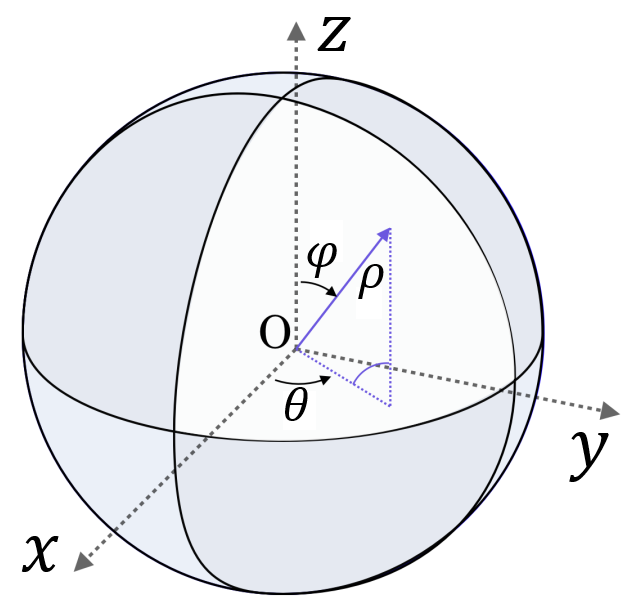
\includegraphics[width=0.2\linewidth]{SphericalCoordinates.png}
\end{figure}

\begin{enumerate}
    \item[$r$] $\geqslant0$ 径向距离
    \item[$\theta$] $\in\left[0,2\pi\right]$ 方位角
    \item[$\varphi$] $\in\left[0,\pi\right]$ 天顶角
\end{enumerate}

\[\left\{\begin{aligned}
        x=x\p{r,\varphi,\theta} & =\rho\sin\varphi\cos\theta \\
        y=y\p{r,\varphi,\theta} & =\rho\sin\varphi\sin\theta \\
        z=z\p{r,\varphi,\theta} & =\rho\cos\varphi           \\
    \end{aligned}\right.\]

\[\iiint_\Omega f\p{x,y,z}\d x\d y\d z=
    \iiint_\Omega f\p{x,y,z}\rho^2\sin\varphi\d\rho\d\varphi\d\theta\]

\subsubsection{曲面面积(可轮换)}

\[\left.\begin{aligned}
        z=z\p{x,y} \\
        \p{x,y}\in D_{xy}
    \end{aligned}\right\}\implies
    S=\iint_{D_{xy}}\sqrt{1+z^{\prime2}_x+z^{\prime2}_y}\d x\d y\]

\subsection{积分应用}

\paragraph{密度为$\rho\p{x,y}$或$\rho\p{x,y,z}$}

\subsubsection{质量}

\[M=\iint_D\rho\p{x,y}\d\sigma,
    M=\iiint_\Omega\rho\p{x,y,z}\d V\]

\subsubsection{质心}

\paragraph{质心的$x$坐标为}

\[\bar x=\frac{\displaystyle\iint_Dx\rho\p{x,y}\d\sigma}M,
    \bar x=\frac{\displaystyle\iiint_\Omega x\rho\p{x,y,z}\d V}M\]

$\rho\p{\cdots}\equiv1$时,质心相当于形心

\subsubsection{转动惯量}

\paragraph{绕$x$轴时}

\[I_x=\iint_Dy^2\rho\p{x,y}\d\sigma,
    I_x=\iiint_\Omega\p{y^2+z^2}\rho\p{x,y,z}\d V\]

\subsubsection{古尔丁定理}

\paragraph{旋转体体积(平面图形$D$绕直线$l:Ax+By+C=0$旋转)}

\[V=\iint_D2\pi d_l\p{x,y}\d\sigma=2\pi\iint_D\frac{\abs{Ax+By+C}}{\sqrt{A^2+B^2}}\d\sigma\]

\subparagraph{若$D$形心为$\p{x_0,y_0}$}

\[V=2\pi d_l\p{x_0,y_0}S_D=2\pi\frac{\abs{Ax_0+By_0+C}}{\sqrt{A^2+B^2}}\iint_D\d\sigma\]


\section{曲线与曲面积分}

\subsection{曲线积分}

\begin{definition}[]
    \[\left\{\begin{aligned}
            x=x\p{r,\theta} & =r\cos\theta \\
            y=y\p{r,\theta} & =r\sin\theta
        \end{aligned}\right.
        \left\{\begin{aligned}
            x & =x\p{t} \\
            y & =y\p{t} \\
            z & =z\p{t}
        \end{aligned}\right.
        \left\{\begin{aligned}
            P & =P\p{x,y,z} \\
            Q & =Q\p{x,y,z} \\
            R & =R\p{x,y,z}
        \end{aligned}\right.\]
\end{definition}

\begin{definition}[第一类]

    $t\in\left[\alpha,\beta\right]$
    $\theta\in\left[\theta_1,\theta_2\right]$

    \[\int_L f\p{x,y}\d s
        =\int^\beta_\alpha f\p{x,y}\sqrt{x^{\prime 2}+y^{\prime 2}}\d t
        =\int_{\theta_2}^{\theta_1}f\p{x,y}\sqrt{r^2+r^{\prime2}}\d\theta\]

    \[\int_\Gamma f\p{x,y,z}\d s
        =\int^\beta_\alpha f\p{x,y,z}\sqrt{x^{\prime 2}+y^{\prime 2}+z^{\prime 2}}\d t\]
\end{definition}

\begin{definition}[第二类(坐标积分)]

    $t:\alpha\to\beta$

    \[\int_LP\d x+Q\d y=
        \int^\beta_\alpha\p{Px^\prime+Qy^\prime}\d t\]

    \[\int_\Gamma P\d x+Q\d y+R\d z=
        \int^\beta_\alpha\p{Px^\prime+Qy^\prime+Rz^\prime}\d t\]
\end{definition}

\subsubsection{格林公式}

\[\oint_LP\d x+Q\d y
    =\iint_D\begin{vmatrix}
        \partial_x & \partial_y \\
        P          & Q
    \end{vmatrix}\d x\d y
    =\iint_D\p{Q^\prime_x-P^\prime_y}\d x\d y\]

\subsubsection{斯托克斯公式}

\[\begin{aligned}
        \oint_\Gamma P\d x+Q\d y+R\d z
         & =\iint_\Sigma\begin{vmatrix}
                            \d y\d z   & \d z\d x   & \d x\d y   \\
                            \partial_x & \partial_y & \partial_z \\
                            P          & Q          & R
                        \end{vmatrix} \\
         & =\iint_\Sigma
        \p{R_y^\prime-Q_z^\prime}\d y\d z+
        \p{P_z^\prime-R_x^\prime}\d z\d x+
        \p{Q_x^\prime-P_y^\prime}\d x\d y
    \end{aligned}\]

\subsubsection{平面曲线积分路径无关条件}

$\int_LP\d x+Q\d y$与积分路径无关

\[\begin{aligned}
             & \int_LP\d x+Q\d y=\int^B_AP\d x+Q\d y \\
        \iff & \oint_LP\d x+Q\d y=0                  \\
        \iff & \exists u=u\p{x,y},\d u=P\d x+Q\d y   \\
        \iff & D\text{内},Q^\prime_x= P^\prime_y
    \end{aligned}\]

\subsubsection{空间曲线积分路径无关}

\[\int_\Gamma P\d y\d z+Q\d z\d x+R\d x\d y\to\left\{\begin{aligned}
        R_y^\prime=Q_z^\prime \\
        P_z^\prime=R_x^\prime \\
        Q_x^\prime=P_y^\prime
    \end{aligned}\right.\]

\subsection{曲面积分}

\begin{definition}[]
    \[z=z\p{x,y}
        \left\{\begin{aligned}
            P & =P\p{x,y,z} \\
            Q & =Q\p{x,y,z} \\
            R & =R\p{x,y,z}
        \end{aligned}\right.\]
\end{definition}

\begin{definition}[第一类(可轮换)]
    \[\iint_\Sigma f\p{x,y,z}\d S=
        \iint_{D_{xy}} f\p{x,y,z}\sqrt{z_x^{\prime 2}+z_y^{\prime 2}+1}\d x\d y\]
\end{definition}

\begin{definition}[第二类(坐标积分)]
    投影到$xOy$坐标面后若所积面与$z$轴方向相同则取正,反之取负

    \[\iint_\Sigma P\d y\d z+Q\d z\d x+R\d x\d y=\pm
        \iint_\Sigma\frac
        {-Pz_x^\prime-Qz_y^\prime+R}
        {\sqrt{z_x^{\prime2}+z_y^{\prime2}+1}}\d S\]
\end{definition}

\subsubsection{三合一投影法}

\[\iint_\Sigma P\d y\d z+Q\d z\d x+R\d x\d y=
    \pm\iint_{D_{xy}}
    \p{-Pz_x^\prime-Qz_y^\prime+R}
    \d x\d y\]

\subsubsection{高斯公式}

\[\oiint_\Sigma P\d y\d z+Q\d z\d x+R\d x\d y=
    \iiint_\Omega\p{P_x^\prime+Q_y^\prime+R_z^\prime}\d V\]

\subsubsection{曲面积分路径无关}

\[\iint_\Sigma P\d y\d z+Q\d z\d x+R\d x\d y
    \to P_x^\prime+Q_y^\prime+R_z^\prime=0\]

\section{向量分析}

\begin{definition}[向量场]
    \[\vec\psi=\left\{P,Q,R\right\}\]
\end{definition}

\subsection{梯度}

\begin{definition}[梯度]
    \[\nabla=\left\{\partial_x,\partial_y,\partial_z\right\}\]
\end{definition}

\subsection{散度}

\begin{definition}[通过$\Sigma$流向指定侧的通量]
    \[\Phi=\iint_\Sigma P\d y\d z+Q\d z\d x+R\d x\d y\]
\end{definition}

\begin{theorem}[散度]
    \[\mathrm{div}\vec\psi=
        \nabla\cdot\vec \psi=
        P_x^\prime+Q_y^\prime+R_z^\prime\]
\end{theorem}

\subsection{旋度}

\begin{definition}[沿封闭曲线$\Gamma$的环流量]
    \[\oint_\Gamma P\d x+Q\d y+R \d z\]
\end{definition}

\begin{theorem}[旋度]
    \[\mathrm{rot}\vec\psi=
        \nabla\times\vec\psi=\left\{
        R_y^\prime-Q_z^\prime,
        P_z^\prime-R_x^\prime,
        Q_x^\prime-P_y^\prime
        \right\}\]
\end{theorem}

\part{空间解析几何}

\section{基础}

\subsection{向量的方向余弦}

\[\boldsymbol v^0=
    \begin{bmatrix}
        \cos\alpha \\
        \cos\beta  \\
        \cos\gamma
    \end{bmatrix}=
    \frac1{\left\Vert\boldsymbol v\right\Vert}
    \begin{bmatrix}\boldsymbol v_x\\\boldsymbol v_y\\\boldsymbol v_z\end{bmatrix}\]

\section{空间曲面}

\subsection{基础}

\begin{definition}[]
    \[F\p{x,y,z}=0\]
\end{definition}

\subsubsection{法向量}

\[\nabla F\]

\subsubsection{方向导数}

方向为$\boldsymbol l$

\[\frac{\partial F}{\partial\boldsymbol l}
    =\partial_xF\cdot\cos\alpha+\partial_yF\cdot\cos\beta+\partial_zF\cdot\cos\gamma
    =\partial_xF\cdot\frac{\boldsymbol l\cdot\boldsymbol i}{\abs{\boldsymbol l}}
    +\partial_yF\cdot\frac{\boldsymbol l\cdot\boldsymbol j}{\abs{\boldsymbol l}}
    +\partial_zF\cdot\frac{\boldsymbol l\cdot\boldsymbol k}{\abs{\boldsymbol l}}\]

\[\boldsymbol l=\nabla F\implies\frac{\partial F}{\partial\boldsymbol l}=\abs{\nabla F}\]

\subsection{平面}

\begin{definition}[]
    \[Ax+By+Cz+D=0\]
\end{definition}

\subsubsection{平面点法式}

过$\p{x_0,y_0,z_0}$,法向量$\begin{bmatrix}A\\B\\C\end{bmatrix}$

\[A\p{x-x_0}+
    B\p{y-y_0}+
    C\p{z-z_0}=0\]

\subsubsection{平面截距式}

\[\frac xa+\frac yb+\frac zc=1\]

\subsubsection{点面距离公式}

点$\p{x_0,y_0,z_0}$

\[d=\frac{\abs{Ax_0+By_0+Cz_0+D}}{\sqrt{A^2+B^2+C^2}}\]

\section{空间曲线}

\begin{definition}[]
    \[\left\{\begin{aligned}
            F\p{x,y,z} & =0 \\
            G\p{x,y,z} & =0
        \end{aligned}\right.\]
\end{definition}

\subsection{参数方程}

\[\left\{\begin{aligned}
        x & =x\p{t} \\
        y & =y\p{t} \\
        z & =z\p{t}
    \end{aligned}\right.\]

\subsection{切向量}

\[\vec\tau=\nabla F\times\nabla G\]

\subsection{直线}

\begin{definition}[]
    \[\left\{\begin{aligned}
            A_1x+B_1y+C_1z+D_1 & =0 \\
            A_2x+B_2y+C_2z+D_2 & =0
        \end{aligned}\right.\]
\end{definition}

\subsection{直线对称式(点向式)方程}

过$\p{x_0,y_0,z_0}$,方向向量$\begin{bmatrix}m\\n\\p\end{bmatrix}$

\[\frac{x-x_0}m=\frac{y-y_0}n=\frac{z-z_0}p=t\]

\subsection{直线参数方程}

\[\left\{\begin{aligned}
        x & =x_0+mt \\
        y & =y_0+nt \\
        z & =z_0+pt
    \end{aligned}\right.\]

\section{特殊曲面}

\begin{definition}[绕$z$轴旋转曲面:(原曲线为$f\p{y_1,z}=0$)]
    \[\left.\begin{aligned}
            f\p{y_1,z}     & =0         \\
            \sqrt{x^2+y^2} & =\abs{y_1}
        \end{aligned}\right\}
        \implies
        f\p{\pm\sqrt{x^2+y^2},z}=0\]
\end{definition}

\subsection{椭圆锥面}

\[\frac{x^2}{a^2}+\frac{y^2}{b^2}=z^2\]

\begin{definition}[以下二次曲面方程中都有]
    \[pq>0\]
\end{definition}

\subsection{椭球面}

\[\frac{x^2}{a^2}+\frac{y^2}{b^2}+\frac{z^2}{c^2}=1\]

\subsection{椭圆抛物面}

\[\frac{x^2}{2p}+\frac{y^2}{2q}=z\]

\subsection{双曲抛物面(马鞍面)}

\[-\frac{x^2}{2p}+\frac{y^2}{2q}=z\]

\[z=xy\]

\subsection{单叶双曲面}

\[\frac{x^2}{a^2}+\frac{y^2}{b^2}-\frac{z^2}{c^2}=1\]

\subsection{双叶双曲面}

\[\frac{x^2}{a^2}+\frac{y^2}{b^2}-\frac{z^2}{c^2}=-1\]

\part{微分方程}

\section{n阶线性微分方程}

\begin{definition}[]
    \[y^{\p{n}}+\sum_{i=0}^{n-1}p_i\p{x}y^{\p{i}}=f\p{x}\label{LinearDifferentialEquationsOfOrderN}\]
\end{definition}

\subsection{线性相关}

\[\frac{f\p{x}}{g\p{x}}=\C(\C\in\sc)\]

\subsection{伯努利方程}

\[y^\prime+P\p{x}y=Q\p{x}y^\alpha\xrightarrow{z=y^{1-\alpha}} z^\prime+\p{1-\alpha}P\p{x}z=\p{1-\alpha}Q\p{x}\]

\subsection{欧拉方程}

\[x^ny^{\p{n}}+\sum_{i=0}^{n-1}p_ix^iy^{\p{i}}=0\]

令$x=\e^t$换元

记$D=\dfrac\d{\d t}$

\[\begin{aligned}
        xy_x^\prime              & =Dy                                                      \\
        x^2y_{xx}^{\prime\prime} & =D\p{D-1}y                                               \\
                                 & \vdots                                                   \\
        x^ny_x^{\p{n}}           & =D\p{D-1}\p{D-2}\cdots\p{D-n+1}y=\prod_{i=1}^n\p{D-i+1}y
    \end{aligned}\]

\section{一阶线性微分方程}

\begin{definition}[$f\p{x}\equiv0$时,为齐次]
    \[\left.\begin{aligned}
            \p{\ref{LinearDifferentialEquationsOfOrderN}} \\
            n=1
        \end{aligned}\right\}
        \implies
        y^\prime+P\p{x}y=f\p{x}\]
\end{definition}

\subsection{通解}

\[y=\frac{\int{f\p{x}\exp\p{\int P\p{x}\d x}\d x}+\C}{\exp\p{\int P\p{x}\d x}}\]

\section{n阶常系数线性齐次微分方程}

\begin{definition}[]
    \[y^{\p{n}}+\sum_{i=0}^{n-1}p_iy^{\p{i}}=0\p{p_i\in\sc}\]
\end{definition}

\subsection{特征方程}

\[r^n+\sum_{i=0}^{n-1}p_ir^i=0\]

\subsection{通解对应项}

\paragraph{$k$重实根$r$在通解中对应项}

\[y_r=\sum_{i=1}^k\C_ix^{i-1}\cdot\e^{rx}\]

\paragraph{特别的:$r$为共轭复根($r=\alpha\pm\beta\i$)时,可改写为两个实根}

\[y_r=(\C_1\cos{\beta x}+\C_2\sin{\beta x})\e^{\alpha x}\]

\section{二阶常系数线性微分方程}

\begin{definition}[]
    \[y^{\prime\prime}+P\p{x}y^\prime+Q\p{x}y=f\p{x}\]
\end{definition}

\subsection{非齐次通解}

\subsubsection{大致形式}

\[y=\underbrace{
        \overbrace{\C_1\overbrace{a\p{x}\e^{r_1x}}^{\text{齐次特解}}+
            \C_2
            \rlap{$\underbrace{\phantom{b\p{x}\e^{r_2x}+x^kc\p{x}\e^{\lambda x}}}_{\text{非齐次特解}}$}
            \overbrace{b\p{x}\e^{r_2x}}^{\text{齐次特解}}}^{\text{齐次通解}}+
        \overbrace{x^kc\p{x}\e^{\lambda x}}^{\text{非齐次特解}}}_{\text{非齐次通解}}\]

\subsubsection{运算关系}

齐特+齐特(线性无关)=齐通

齐通+非特=非通

齐特+非特=非特

非特$-$非特=齐特

\subsection{齐次微分方程}

\begin{definition}[]
    \[y^{\prime\prime}+py^\prime+qy=0\]
\end{definition}

\subsubsection{特征方程}

\[r^2+pr+q=0\]

\subsubsection{通解}

\paragraph{$r_1\neq r_2$}

\[y=\C_1\e^{r_1x}+\C_2\e^{r_2x}\]

\paragraph{$r_1=r_2$}

\[y=\p{\C_1+\C_2x}\e^{r_1x}\]

\paragraph{$r_{1,2}=\alpha\pm\beta\i$}

\[y=(\C_1\cos{\beta x}+\C_2\sin{\beta x})\e^{\alpha x}\]

\subsection{非齐次微分方程}

\begin{definition}[]
    \[y^{\prime\prime}+py^\prime+qy=f\p{x}\label{LinearDifferentialEquationsWithSecondOrderConstantCoefficients}\]
\end{definition}

\subsubsection{特解}

$\mathcal P_n$表示$n$次多项式

\[\left.\begin{aligned}
               & \p{\ref{LinearDifferentialEquationsWithSecondOrderConstantCoefficients}}                            \\
        f\p{x} & =\left[\mathcal P_{n_1}\p{x}\cos{\omega x}+\mathcal P_{n_2}\p{x}\sin{\omega x}\right]\e^{\lambda x} \\
        m      & =\max{\left\{n_1,n_2\right\}}
    \end{aligned}\right\}
    \implies\]

\[y^*=x^k\left[\mathcal U_m\p{x}\cos{\omega x}+\mathcal V_m\p{x}\sin{\omega x}\right]\e^{\lambda x}
    \left\{\begin{aligned}
         & k=0 & \p{\lambda\pm\omega \i\text{不是特征方程根}} \\
         & k=1 & \p{\lambda\pm\omega \i\text{是特征方程根}}
    \end{aligned}\right.\]

当$\omega=0$时,$m=n_1$

\[\left.\begin{aligned}
         & \p{\ref{LinearDifferentialEquationsWithSecondOrderConstantCoefficients}} \\
         & f\p{x}=\mathcal P_m\p{x}\e^{\lambda x}
    \end{aligned}\right\}
    \implies
    y^*=x^k\mathcal Q_m\p{x}\e^{\lambda x}
    \left\{\begin{aligned}
        k=0 &  & \p{\lambda\text{不是特征方程根}} \\
        k=1 &  & \p{\lambda\text{是特征方程单根}} \\
        k=2 &  & \p{\lambda\text{是特征方程重根}}
    \end{aligned}\right.\]

\subsubsection{算子法求特解}

\begin{definition}[$D$算子]
    \[Df\p{x}=f^\prime\p{x},\frac1Df\p{x}=\int f\p{x}\d x\]
\end{definition}

对于$\p{\ref{LinearDifferentialEquationsWithSecondOrderConstantCoefficients}}$:

\[y^*=\frac1{D^2+pD+q}f\p{x}=\frac1{\mathcal F\p{D}}f\p{x}\]

若代入$D$后分母$\mathcal F\p{D}$出现为$0$的状况,则(可多次使用,$D$算子只对右侧$f\p{x}$有效):

\[y^*=x^n\frac1{\mathcal F\p{D}}f\p{x}\longrightarrow y^*=x^{n+1}\frac1{\mathcal F^\prime\p{D}}f\p{x}\]

\paragraph{$f\p{x}=\e^{kx}$:$D$换为$k$}

\[y^*=\frac1{\mathcal F\p{D}}\e^{kx}=\frac1{\mathcal F\p{k}}\]

\paragraph{$f\p{x}=\sin ax$或$\cos ax$:$D^2$换为$-a^2$}

若代入$D^2$后,分母有$mD+n\p{mn>0}$一次多项式,可以配平方将一次多项式化到分子,再代入$D^2$后直接使用$D$算子求导

\paragraph{$f\p{x}=\mathcal P_n\p{x}$:}

使用$\dfrac1{1-x}=\sum\limits_{n\in\sn}x^n$泰勒展开$\dfrac1{\mathcal F\p{D}}$(不考虑收敛域),
使得展开后$D$的最高次幂不小于$\mathcal P_n\p{x}$即可

若$\mathcal F\p{D}$不含常数项,则先提出$\dfrac1D$

展开时将$1-\mathcal F\p{D}$当作$x$,但$1-\mathcal F\p{D}$中不应含有常数项,形如:

\[\frac1{D^2+pD+q}=\frac1q\cdot\frac1{1+\frac{D^2+pD}q}\]

\paragraph{$f\p{x}=\e^{kx}y\p{x}$:移位定理}

\[y^*=\frac1{\mathcal F\p{D}}\e^{kx}y\p{x}=\e^{kx}\frac1{\mathcal F\p{D+k}}y\p{x}\]

\paragraph{$f\p{x}=\mathcal P_n\p{x}\sin ax$:}

\[y^*=\frac1{\mathcal F\p{D}}\mathcal P_n\p{x}\sin ax=\Im\left[{\frac1{\mathcal F\p{D}}\mathcal P_n\e^{\i ax}}\right]\]

\paragraph{$f\p{x}=\mathcal P_n\p{x}\cos ax$:}

\[y^*=\frac1{\mathcal F\p{D}}\mathcal P_n\p{x}\cos ax=\Re\left[{\frac1{\mathcal F\p{D}}\mathcal P_n\e^{\i ax}}\right]\]

\section{全微分方程}

\subsection{条件(微分换序)}

\[P\p{x,y}\d x+Q\p{x,y}\d y=0\text{是全微分方程}\iff P_y^\prime=Q_x^\prime\]

\part{无穷级数}

\section{收敛与发散}

\subsection{绝对收敛}

\[\sum_{n\in\snp}\abs{u_n}=s,s\in\sc\]

且$\sum\limits_{n\in\snp}u_n$一定收敛

\subsection{条件收敛}

\[\sum_{n\in\snp}u_n=s,\sum_{n\in\snp}\abs{u_n}\text{发散},s\in\sc\]

\[\text{绝对收敛}\cap\text{条件收敛}=\emptyset\]

\subsection{运算关系}

收敛 + 收敛 = 收敛

收敛 + 发散 = 发散

发散 + 发散 = 不确定

绝对收敛 + 绝对收敛 = 绝对收敛

绝对收敛 + 条件收敛 = 条件收敛

条件收敛 + 条件收敛 = 收敛(不确定条件还是绝对)

绝对收敛 $\times$ 条件收敛 = 绝对收敛

\subsection{无穷大比较}

\[n\to+\infty\]

\[n^n\gg n!\gg a^n\p{a>1}\gg n^p\p{p>1}\gg |\gg n^p\p{1\geqslant p>0}\gg\p{\ln n}^q\p{q>0}\]

$\displaystyle\sum_{n\in\snp}\frac1{u_n}$中,若$u_n$在$|$记号左侧则收敛,在$|$记号右侧则发散

$\displaystyle\sum_{n\in\snp}\frac{v_n}{u_n}$中,若$u_n$在$|$记号左侧,且$v_n$在$u_n$右侧时收敛,否则发散
($\dfrac{n^p\p{1\geqslant p>0}}{n^q\p{q>1}}$除外,需进一步$p>q+1$才收敛)

\section{任意项级数}

\subsection{比值审敛法(达朗贝尔判别法)}

\[\lim_{n\to\infty}\abs{\frac{u_{n+1}}{u_n}}
    \left\{\begin{aligned}
         & <1 & \implies & \sum u_n\text{绝对收敛}     \\
         & =1 & \implies & \sum u_n\text{可能收敛可能发散} \\
         & >1 & \implies & \sum u_n\text{发散}
    \end{aligned}\right.\]

\subsection{根值审敛法(柯西判别法)}

\[\lim_{n\to\infty}\sqrt[n]{\abs{u_n}}
    \left\{\begin{aligned}
         & <1 & \implies & \sum u_n\text{绝对收敛}     \\
         & =1 & \implies & \sum u_n\text{可能收敛可能发散} \\
         & >1 & \implies & \sum u_n\text{发散}
    \end{aligned}\right.\]

\section{正项级数}

收敛$\iff$绝对收敛

\subsection{积分审敛法}

\[\sum_{n\in\snp}f\p{n}\text{敛散同}
    \int_1^{+\infty}f\p{x}\d x\]

\subsection{比较审敛法}

大收敛则小收敛,小发散则大发散

\[\lim_{n\to\infty}\frac{u_n}{v_n}
    \left\{\begin{aligned}
         & =0               & \implies & \sum v_n\text{收敛}\Rightarrow\sum u_n\text{收敛},\sum u_n\text{发散}\Rightarrow\sum v_n\text{发散} \\
         & \in\p{0,+\infty} & \implies & \sum v_n\text{敛散同}\sum u_n                                                                  \\
         & =+\infty         & \implies & \sum v_n\text{发散}\Rightarrow\sum u_n\text{发散},\sum u_n\text{收敛}\Rightarrow\sum v_n\text{收敛}
    \end{aligned}\right.\]

\section{交错级数}

\subsection{莱布尼兹判别法}

\[\left.\begin{aligned}
        \text{正项级数}u_n\searrow \\
        \lim_{n\to\infty}u_n=0
    \end{aligned}\right\}
    \implies
    \text{交错级数}\sum\p{-1}^{n\text{(或}n-1\text{)}}u_n\text{收敛}\]

\section{幂(泰勒)级数}

\begin{definition}[以下默认幂级数形式]

    \[\sum_{n\in\sn}a_nx^n,\text{收敛半径为}R\]

\end{definition}

\subsection{阿贝尔定理}

\[\left\{\begin{aligned}
         & \abs{x}<R &  & \text{绝对收敛}         \\
         & \abs{x}=R &  & \text{单独讨论(可能条件收敛)} \\
         & \abs{x}>R &  & \text{发散}
    \end{aligned}\right.\]

收敛区间为$\p{-R,R}$,收敛域需要讨论端点$\abs{x}=R$处的值

\subsection{系数模比值法}

\[\lim_{n\to\infty}\abs{\frac{a_{n+1}}{a_n}}=\rho\implies R=\frac1\rho\]

\subsection{系数模根值法}

\[\lim_{n\to\infty}\sqrt[n]{\abs{a_n}}=\rho\implies R=\frac1\rho\]

\subsection{加减运算}

\[\left.\begin{aligned}
        \sum a_nx^n\text{收敛域为}I_a \\
        \sum b_nx^n\text{收敛域为}I_b
    \end{aligned}\right\}
    \implies\sum a_nx^n\pm\sum b_nx^n=\sum\p{a_n\pm b_n}x^n,x\in I_a\cap I_b\]

\subsection{求导积分运算}

幂级数求导、积分后,收敛半径不变

求导后,收敛域可能缩小(边界点可能发散)

积分后,收敛域可能扩大(边界点可能收敛)

\subsection{泰勒级数}

\[f\p{x}\sim
    \sum_{n\in\sn}\frac{f^{\p{n}}\p{x_0}}{n!}\p{x-x_0}^n\]

\subsection{常用泰勒级数\label{Taylor}}

\[\newcommand{\series}[1]{\sum_{n\in#1}}
    \begin{aligned}
        \e^x           & =1+x+\frac{x^2}{2!}+\frac{x^3}{3!}+o\p{x^3}           &  & =\series\sn\frac{x^n}{n!}                                  &                              \\
        \sin x         & =x-\frac{x^3}{3!}+\frac{x^5}{5!}+o\p{x^5}             &  & =\series\sn\p{-1}^n\frac{x^{2n+1}}{\p{2n+1}!}              &                              \\
        \cos x         & =1-\frac{x^2}{2!}+\frac{x^4}{4!}+o\p{x^4}             &  & =\series\sn\p{-1}^n\frac{x^{2n}}{\p{2n}!}                  &                              \\
        \tan x         & =x+\frac13x^3+\frac2{15}x^5+o\p{x^5}                  &  & =\series\snp\frac{B_{2n}\p{-4}^n\p{1-4^n}}{\p{2n}!}^{2n-1} & x\in\p{-\frac\pi2,\frac\pi2} \\
        \arctan x      & =x-\frac{x^3}3+\frac{x^5}5+o\p{x^5}                   &  & =\series\sn\frac{\p{-1}^n}{2n+1}x^{2n+1}                   & x\in\left[-1,1\right]        \\
        \arcsin x      & =x+\frac16x^3+\frac3{40}x^5+o\p{x^5}                  &  & =\series\sn\frac{\p{2n}!}{4^n\p{n!}^2\p{2n+1}} x^{2n+1}    & x\in\p{-1,1}                 \\
        \ln\p{1+x}     & =x-\frac{x^2}2+\frac{x^3}3+o\p{x^3}                   &  & =\series\snp-\frac{{\p{-x}}^n}n                            & x\in\left(-1,1\right]        \\
        \ln\p{1-x}     & =-x-\frac{x^2}2-\frac{x^3}3+o\p{x^3}                  &  & =\series\snp-\frac{x^n}n                                   & x\in\left(-1,1\right]        \\
        \frac1{1+x}    & =1-x+x^2-x^3+o\p{x^3}                                 &  & =\series\sn\p{-x}^n                                        & x\in\p{-1,1}                 \\
        \frac1{1-x}    & =1+x+x^2+x^3+o\p{x^3}                                 &  & =\series\sn x^n                                            & x\in\p{-1,1}                 \\
        \p{1+x}^\alpha & =1+\alpha x+\frac{\alpha\p{\alpha-1}}{2!}x^2+o\p{x^2} &  & =\series\sn\binom\alpha nx^n                               & x\in\p{-1,1}
    \end{aligned}\]

\section{三角(傅里叶)级数}

\subsection{傅里叶级数}

\[f\p{x}\sim\frac{a_0}2+\sum_{n\in\snp}\p{a_n\cos\frac{n\pi x}l+b_n\sin\frac{n\pi x}l}\]

$f\p{x}$周期为$T=2l$时($l$常取$\pi$),有傅里叶系数:

\[\left\{\begin{aligned}
        a_n & =\frac1l\int_{-l}^lf\p{x}\cos\frac{n\pi x}l\d x,n\in\sn  \\
        b_n & =\frac1l\int_{-l}^lf\p{x}\sin\frac{n\pi x}l\d x,n\in\snp
    \end{aligned}\right.\]

\[\omega=\frac{2\pi}T=\frac\pi l\]

\subsection{特殊情况}

\subsubsection{正弦级数}

若$f\p{x}$是在一个周期上是奇函数,则$a_n=0$

\[f\p{x}\sim\sum_{n\in\snp}b_n\sin\frac{n\pi x}l\]

\subsubsection{余弦级数}

若$f\p{x}$是在一个周期上是偶函数,则$b_n=0$

\[f\p{x}\sim\frac{a_0}2+\sum_{n\in\snp}a_n\cos\frac{n\pi x}l\]

\subsection{狄利克雷收敛定理}

$f\p{x}$在一个周期内有:

\begin{enumerate}
    \item 连续或只有有限个第一类间断点
    \item 只有有限个极值点
\end{enumerate}

即$f\p{x}$的傅里叶级数在$\sr$连续,且

\begin{enumerate}
    \item $x_0$连续时,级数收敛于$f(x_0)$
    \item $x_0$是第一类间断点时,级数收敛于$\dfrac{f(x_0^-)+f(x_0^+)}2$
\end{enumerate}

\end{document}
